\end{multicols}
\begin{multicols}{2}[\section{Implementation}]
\label{sec:implementation}

The Implementation section covers certain issues regarding implementation tasks. Problems and their solutions will be discussed.


\end{multicols}
\begin{multicols}{2}[\subsection{Data access layer}]

For implementing the data access layer we defined code-templates which were simply filled with values, according to our XML schema definition – much like a serial letter. While tedious in the beginning (since the code-templates are written in XML) we quickly became used to it. Since all classes are built from the same template, it was quite easy fix bugs once and for all.

It also proved to be a quite extendable concept. For example, it took us just a few hours to implement a query cache, which increased the speed of the scheduler about 8 times. Once the API was defined, it was easy to enhance performance without putting the stability of the rest of our code base at risk.

We chose to use Java SEs native SQL-API from the java.sql-package to access the database. Thanks to the use of prepared statements we did not have any trouble with malformed user inputs, making our software virtually invulnerable against things such as SQL injections.

\raggedcolumns
\columnbreak

\paragraph{Use of AspectJ and PL/pgSQL} One of the most compelling features of automatically generating code is, that changes made to the template are reflected in all derived classes. However, it comes at a cost. One can not manually edit that code, without either loosing the advantage of automatically adapting changes or loosing the extensions made manually. Thus we used AspectJ to \emph{cross-cut} the auto-generated classes and so implement special functionality. Using PL/pgSQL these functions were implemented efficiently within the database, taking full advantage of PostgreSQL’s rich set of server-side programming features.

An example for this is the enrollment in courses. To enroll a student into a course (actually a course instance) many requirements have to be checked (whether a user has passed required courses, whether there are enough free seats, etc.). This function was implemented in the database and included into the Java class \emph{CourseInstancce} using an Aspect named \emph{Enrollment}, which introduces the method \emph{enroll(Person p)} in that class.

\paragraph{PostgreSQL-specific issues} The most trouble we had were annoyances and inconsistencies between the promises of the Java SQL API and the implementation of it in the PostgreSQL-JDBC-Driver. For example, \texttt{java.sql.Statement.getGeneratedKeys()} returns any auto-generated keys during the last query. However, the implementation of the PostgreSQL-Driver does not support that feature and so we had to work around this short coming using a PostreSQL-specific language extension.


\end{multicols}
\begin{multicols}{2}[\subsection{Controller}]

In order to implement the Controller and associated interfaces as described in the design section, we had to utilize Javas Reflection API. Problems we faced arose mostly from Javas Type System, especially Generics, which proved to be quite cumbersome to work with.

\paragraph{OutputConverter} Thanks to a clean design it was easier than we thought at first to implement a multitude of different \emph{OutputConverter}. Thus we created a whole lot of them, for XHTML, HTML5 as well as PDF and even text/plain Output.

\paragraph{Shared Code} Since many functions were the same across many different modules in the business layer, we created common abstract classes for shared functionality.


\begin{figure}[H]
	\centering
		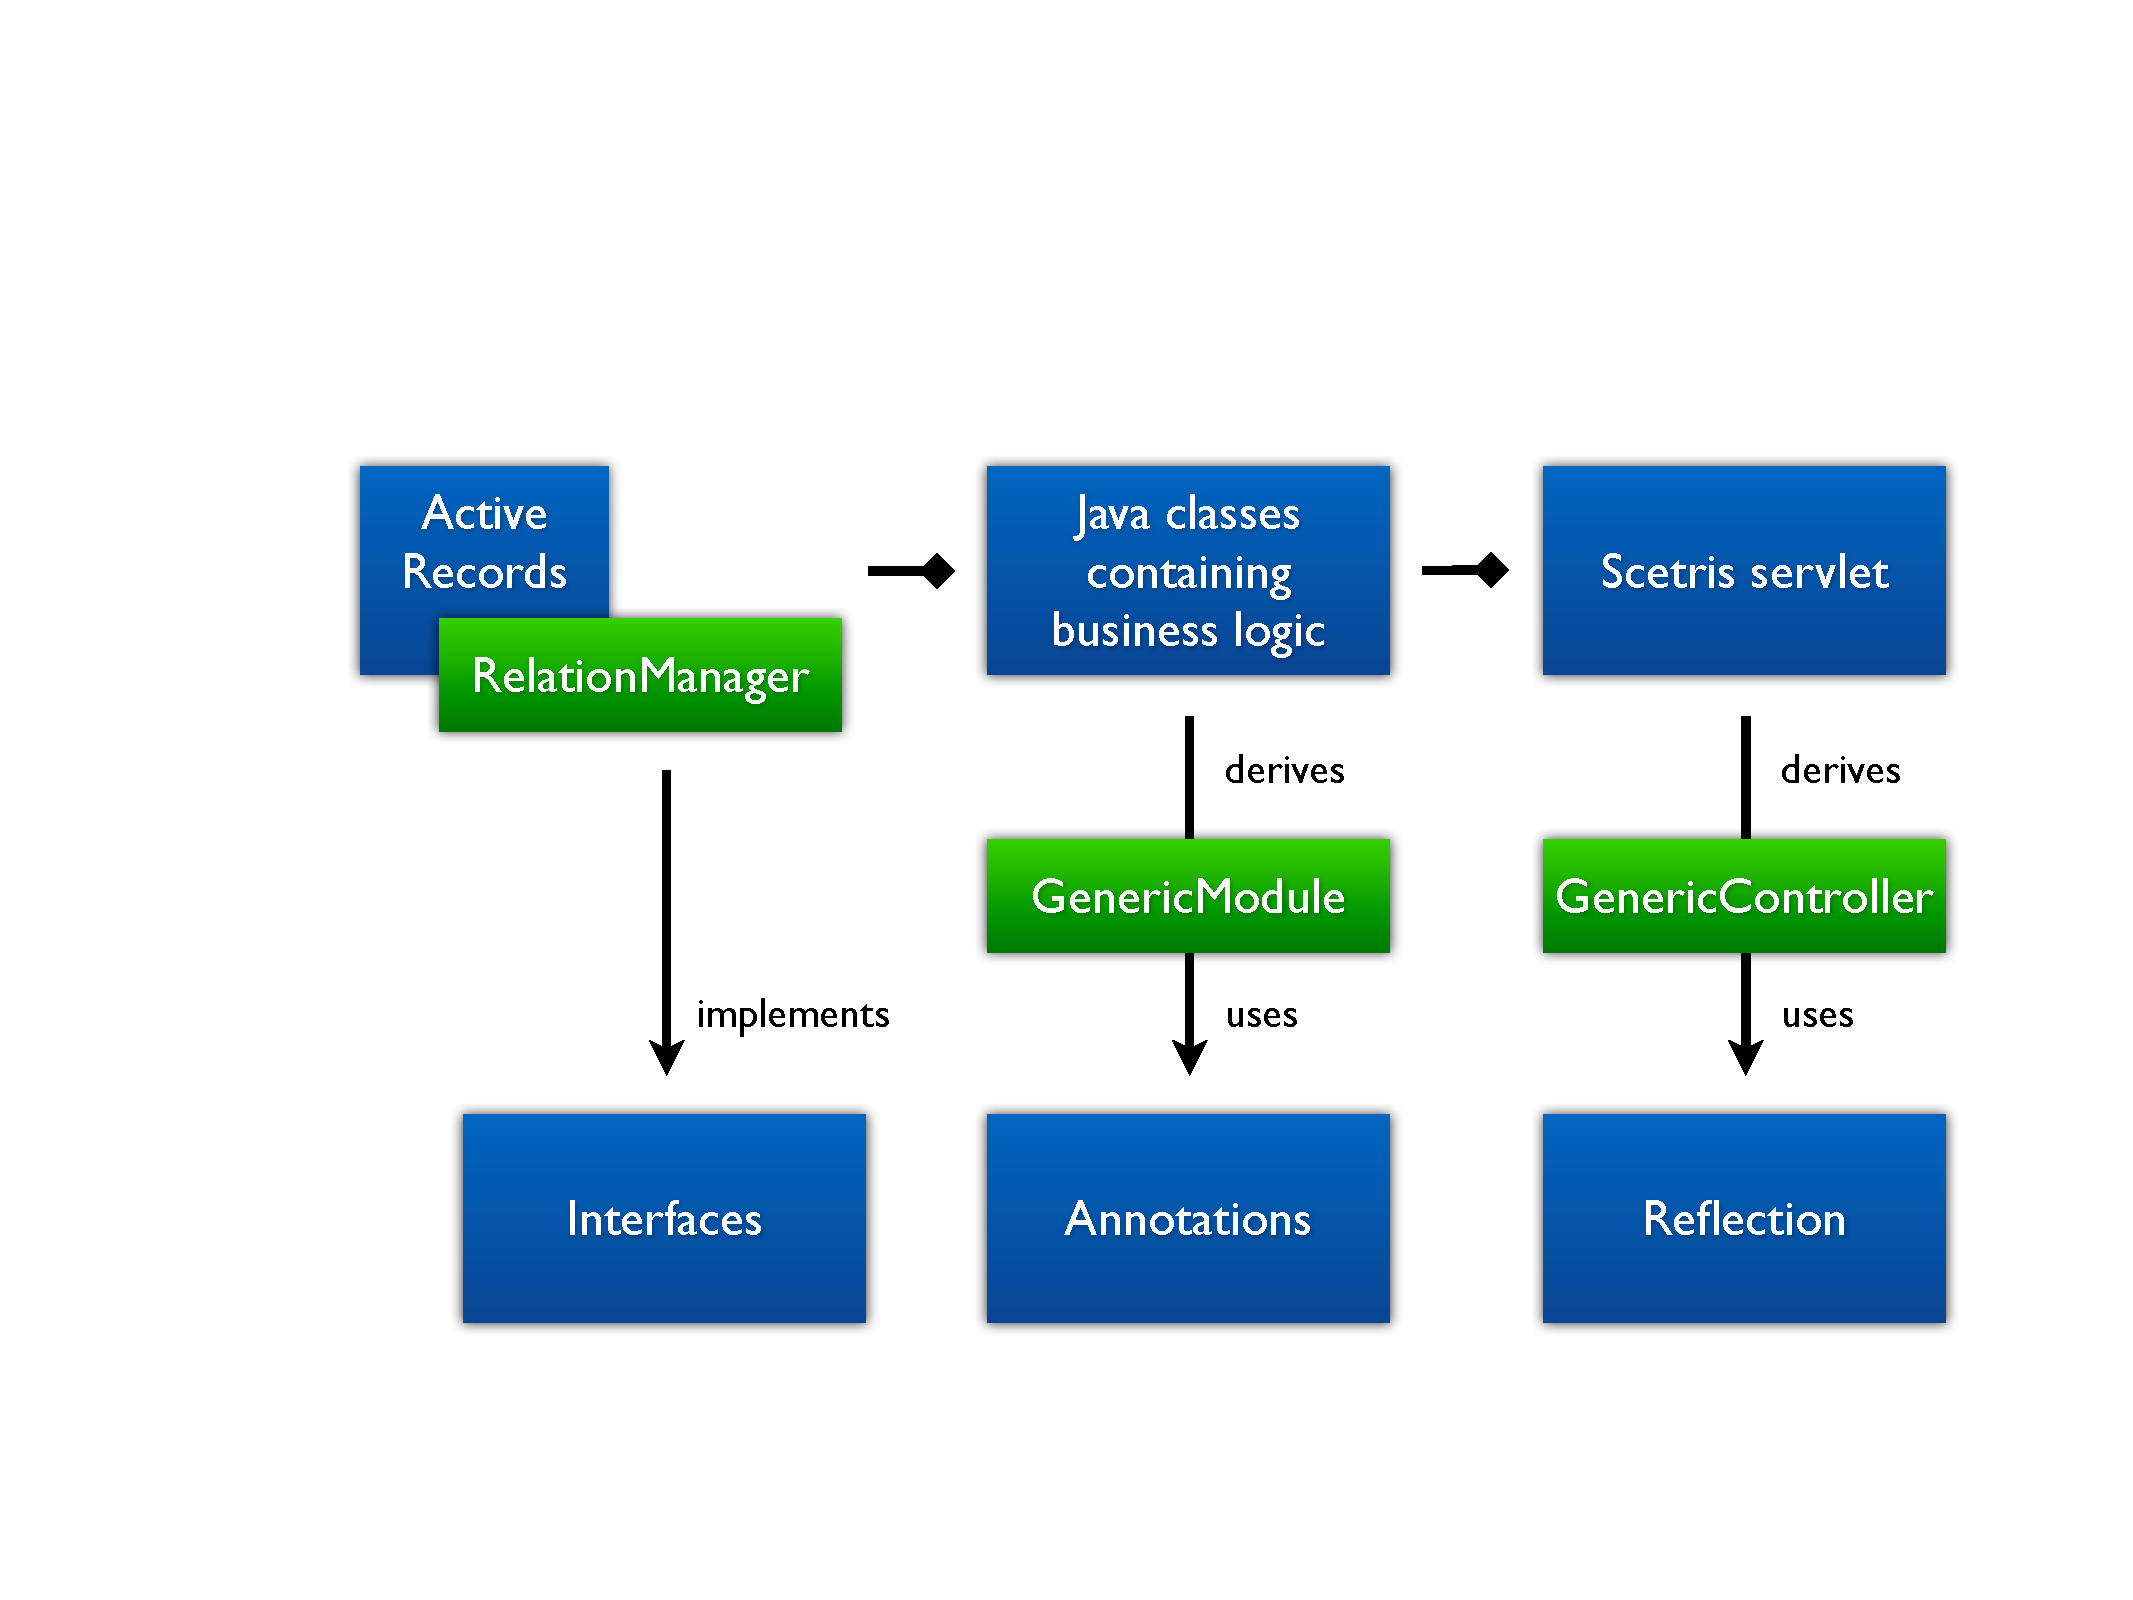
\includegraphics[width=\columnwidth]{images/web-classes.pdf}
	\caption{Composition of business logic, controlling logic and data access layer.}
	\label{fig:scheduler}
\end{figure}


\end{multicols}
\begin{multicols}{2}[\subsection{Front end / Templates}]

The front end was implemented using XSL-T templates. The main idea was to make it easier for us to build the web application. To do so we created lego-bricks -- as we called them -- our main form building mechanism. It simplified the work in a way, that we just handled little data into the templates and got rich, unified forms in return. As a result we did not need to bother about layout and style, since the templates always created HTML which looked similar, thus a uniform look and feel of the site.


\end{multicols}
\begin{multicols}{2}[\subsection{Scheduler}]

The major problem of implementing a genetic algorithm is the question of how to represent the solutions. The genetic algorithm operations presented can only be applied when a fitting data model has been designed. Traditionally an array is used. The \emph{crossover} operation applied on two candidate solutions leads to mixing these values with each other. The \emph{mutation} operation on one candidate solution leads to randomly changing values of the array.

A generic approach to solve this problem is to encode the data model into a byte representation. But since we had chosen AspectJ respectively Java to implement the scheduler we wanted to use the concept of object-orientied programming and all its advantages. Fortunately there was a reference solution\link{http://www.codeproject.com/KB/recipes/GaClassSchedule.aspx}{Homepage of The Code Project with example implementation of genetic algorithm} implemented in C++, which we based our implementation on. The candidate solutions are represented by using a \emph{Map}.

\[CourseElementInstance \mapsto (Room,Time Slot)\]

Every course is mapped to a tuple defined by a room and a time slot. The time slot is the starting time slot of the course [Figure \ref{fig:map}].

\raggedcolumns
\columnbreak

\begin{figure}[H]
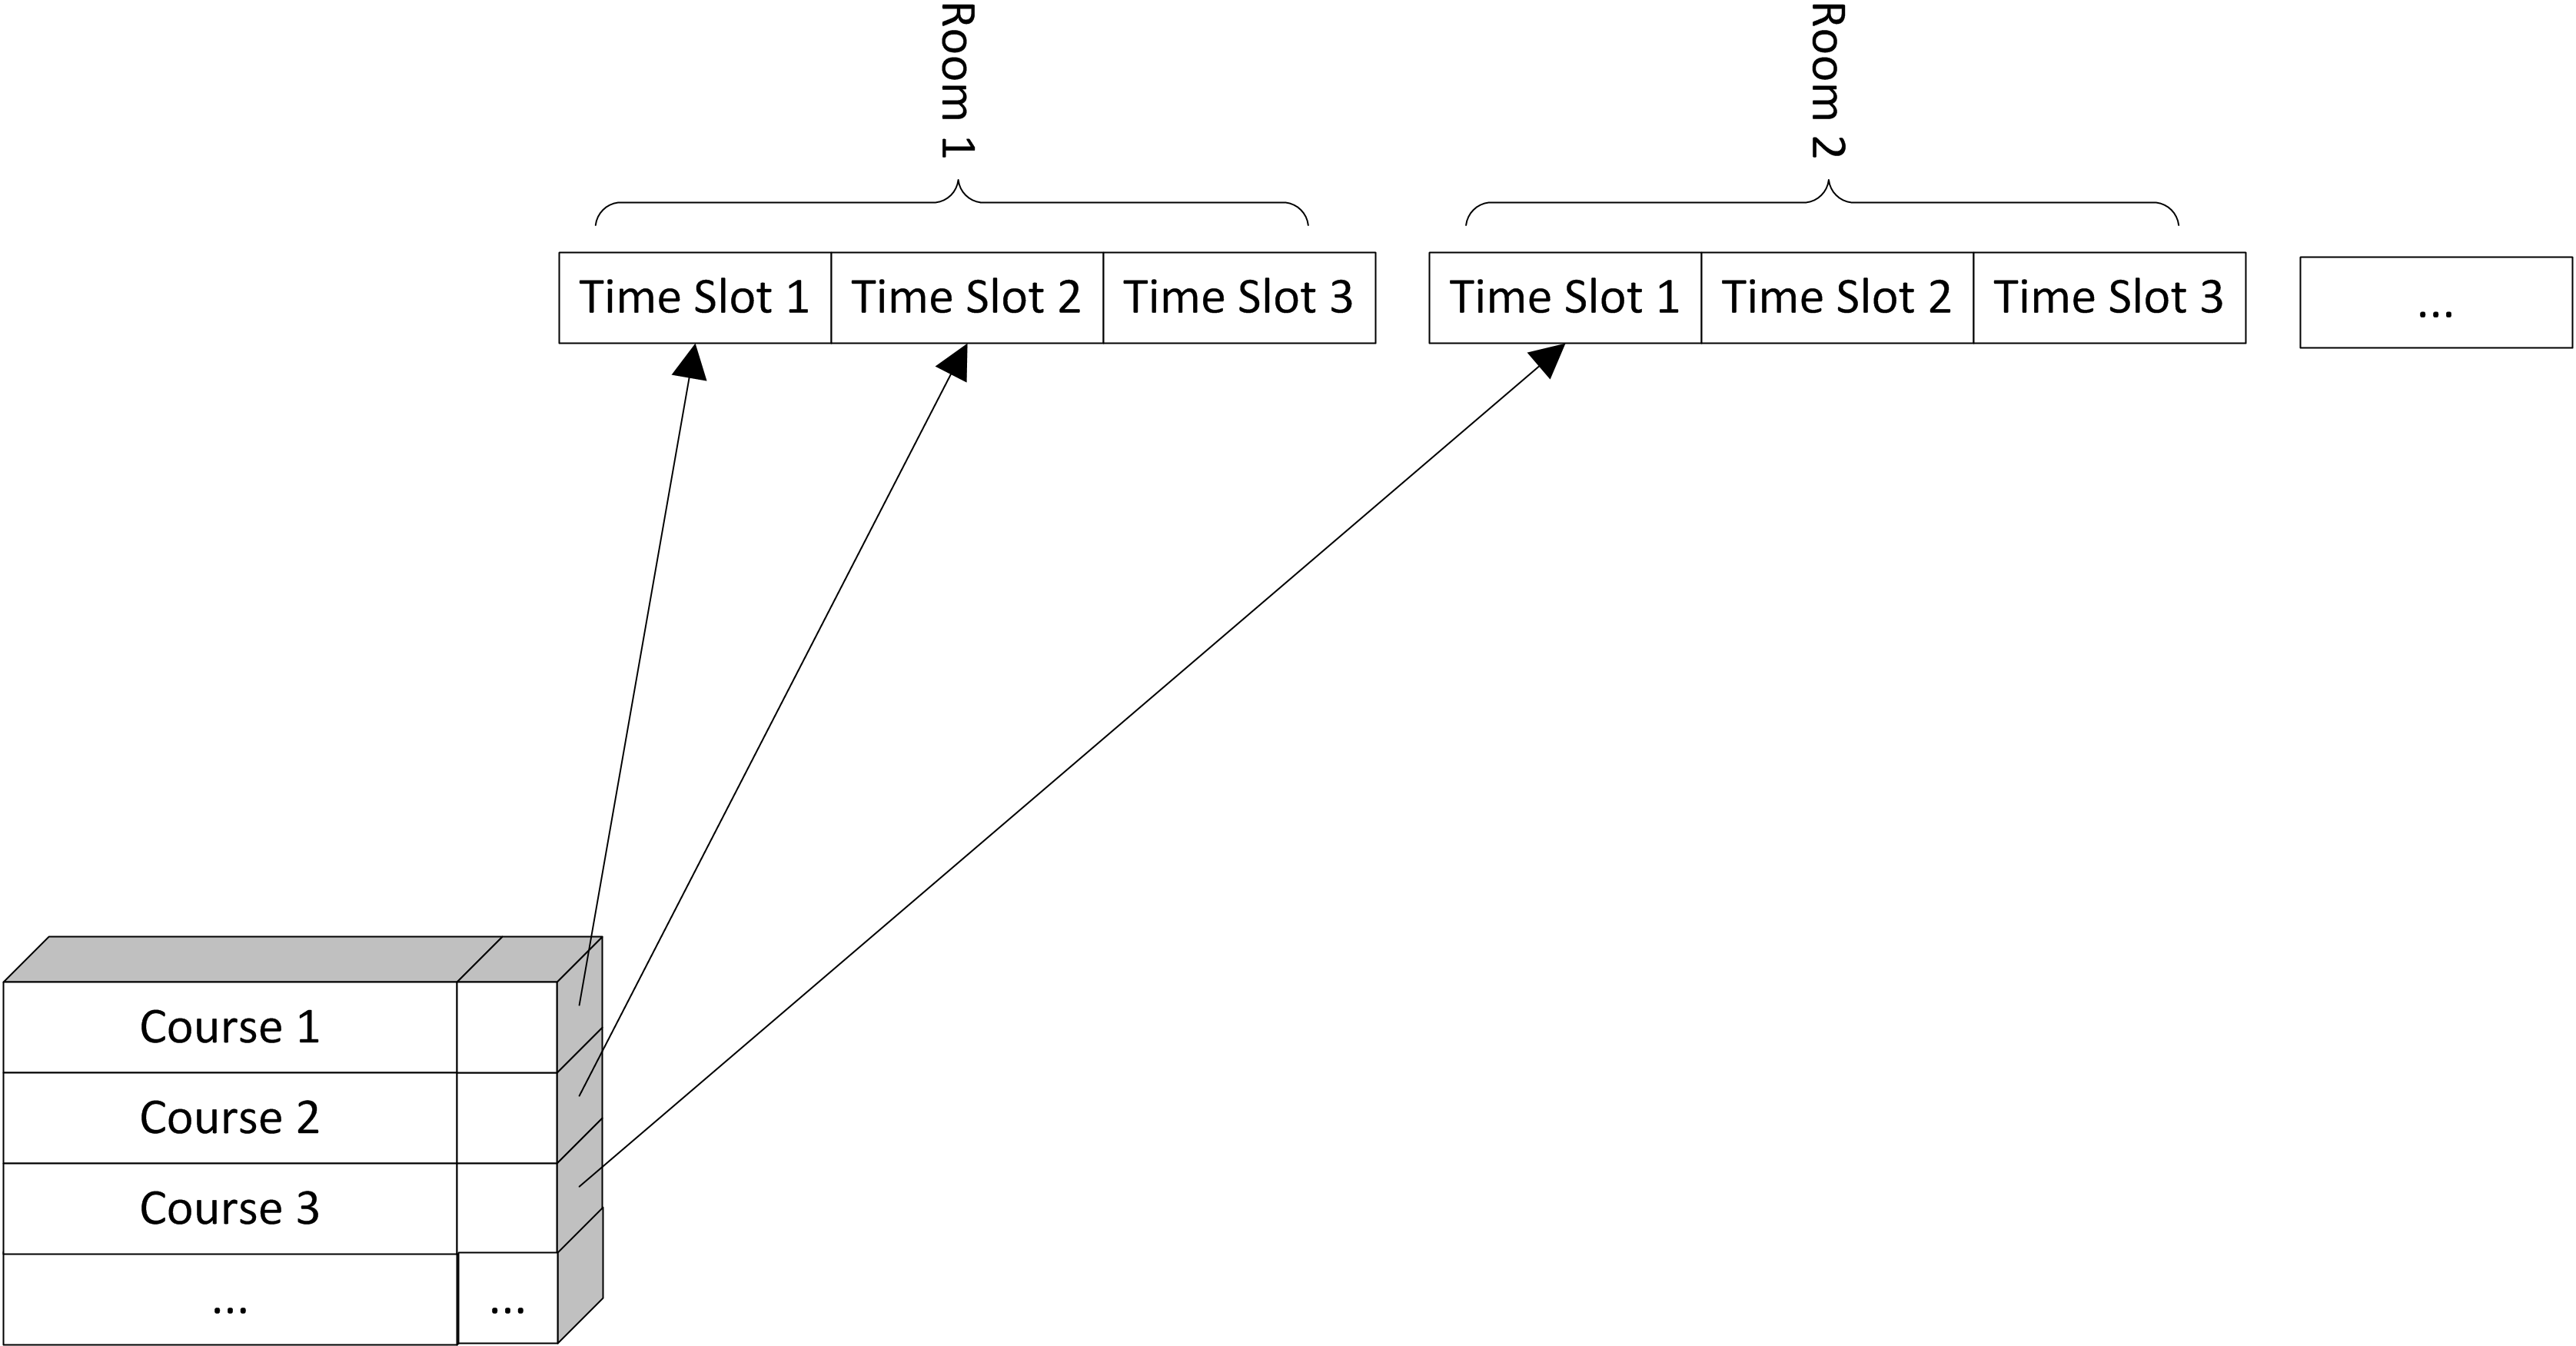
\includegraphics[width=\columnwidth]{images/map.png}%
\caption{Every Course is mapped to a tuple defined by a room and a time slot.}%
\label{fig:map}%
\end{figure}

 As a matter of fact this is not sufficient to model the whole candidate solution. Behind this data model lies another data model modeling the whole timetable. The data model is a list of rooms with each having a further list with time slots. On every time slot there is another list with courses allocated to this position. Instead of a single course a list of courses was chosen because there is the possibility of having one course in the same room at the same time.

\[ [(Room,[(TimeSlot,[CourseElementInstance])] \]

However, applying \emph{crossover} and \emph{mutation} only takes effect on the \emph{Map}. An example of executing \emph{crossover} on the designed data model is illustrated in Figure \ref{fig:data-model}.

\begin{figure}[H]
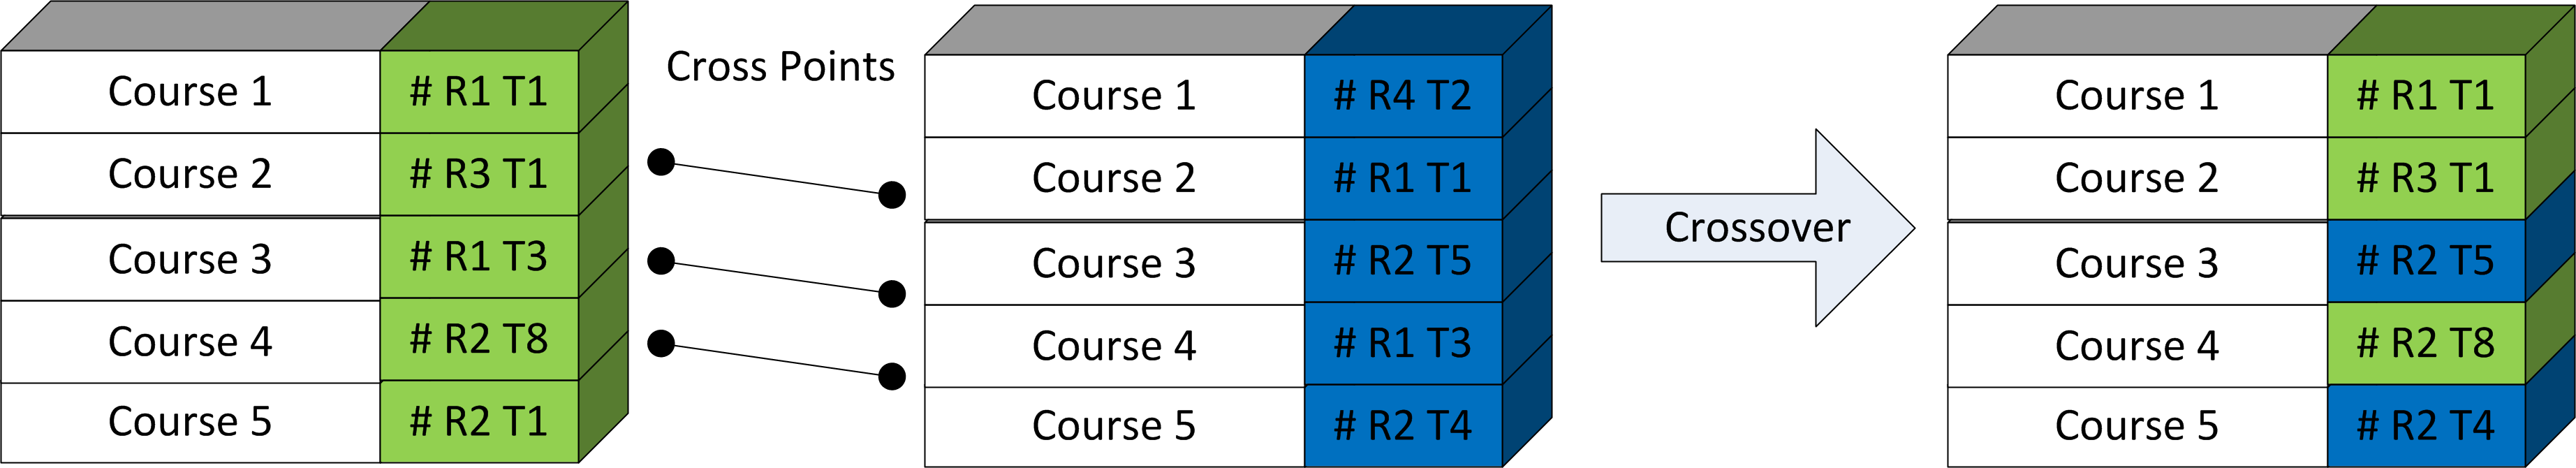
\includegraphics[width=\columnwidth]{images/crossover.png}
\caption{Crossover operation: A specified amount of cross points is chosen randomly. The courses are iterated and taken over to the offspring candidate solution. When a cross point is met the other candidate solution being crossed over is used to take over its course allocations.}
\label{fig:data-model}
\end{figure}

In the implementation phase it turned out using a \emph{setup} allocating the course completely random works for little input very well. With increased input, however, the results by  the classical \emph{setup} lead to quite worse results. These results are supposed to be optimized by the phase of applying \emph{crossover} and \emph{mutate}. As a matter of fact this happens to a certain degree but starts to converge to a certain score.

Therefore an alternative \emph{setup} was implemented. \emph{Greedy setup} combines the approach of a genetic algorithm using metaheuristic with the Greedy algorithm being a subset of the combinatorial algorithm.

\begin{description}
\item[Greedy Setup] generates the initial population of candidate solutions by using a Greedy algorithm. Every course is allocated by placing it to the room which fits its constraints best, for instance the requirement for a specified amount of seats. In order to avoid choosing rooms which exceed the required constraints every room is rated and sorted. In order to avoid overlapping in space and time the courses are placed one after another in the timetable.
\end{description}

There is the possibility of finding an optimal solution in the phase of \emph{Greedy setup}. Therefore the \emph{fitness function} is applied on every generated candidate solution. If an optimal schedule has been found the algorithm terminates.
